\documentclass{beamer}

\mode<presentation>{
    \usetheme{presentationleria}
}

%%%%%%%%% Packages obligatoires
\usepackage{lmodern}
\usepackage[T1]{fontenc}
\usepackage[utf8]{inputenc}
\usepackage[francais]{babel}
\usepackage{graphicx}
\usepackage{chronosys}%frise chronologique
\usepackage{color}
\usetikzlibrary{matrix,backgrounds}%matrice
\usetikzlibrary{arrows.meta}
\usepackage{comment} 
\usepackage[french,onelanguage,ruled,vlined]{algorithm2e}%algo
\usepackage{colortbl}
\usepackage{geometry}
\usepackage{datenumber,xparse}
\usepackage{tcolorbox,listings}%listing bibli

\usepackage{graphicx}
\usepackage{color}
\usepackage{xcolor}
\usepackage[french,onelanguage,ruled,vlined]{algorithm2e}%algo
%\usepackage{hyperref}%doublon
\usepackage{array}
\usepackage{transparent}
\usepackage{float}
%\input{img/setXml}
\usepackage[style=numeric,sorting=none]{biblatex}
\addbibresource{references.bib}

%%%%%%%%% Informations sur le document
\author[C. Behuet]{
%\textbf{Corentin Behuet}\\
%~\\
\textbf{JFPC 2022}\\
V. Barichard,\textbf{ C.Behuet}, D. Genest, M. Legeay, D. Lesaint\\
\textit{Laboratoire d’étude et de recherche en informatique d’Angers (LERIA)}\\ 
%~\\
%Thèse financée par l'Université d'Angers et le projet Thélème
%\textit{Thèse cofinancée par le projet Thélème
%octroyé aux universités d’Angers et du Mans dans le cadre
%du PIA3}
}
\institute[LERIA]{}
\titlegraphic{
  \hfill
  
\includegraphics[width=0.2\textwidth]{logos/logo_leria.pdf}
  \hfill
  
\includegraphics[width=0.25\textwidth]{logos/ua_h_couleur_ecran.png}
  \hfill
  ~
}
% Titre :   M. Legeay,  
\title[Conception d'emplois du temps universitaires ]{Approche par contraintes\\ pour une classe d’emplois du temps universitaires}

%\subtitle{Journée du LERIA 2021}
% Date (\today ou une date) :
\date{}
% Nom à affiche pour le plan (Plan, Sommaire, etc.) :
\newcommand{\nomplan}{Sommaire}

%%%%%%%%% Plan automatique
% Section
\AtBeginSection{\plansection}
% Sous-section
\AtBeginSubsection{\plansoussection}

\begin{document}

\begin{frame}
    \titlepage
    
\end{frame}

\begin{frame}
\frametitle{\nomplan}
\tableofcontents
\end{frame}

%=============================

\section{Problématique des EDT universitaires}

\begin{frame}{Processus de construction d'EDT}

\begin{itemize}
\centering
\item Focus sur le système universitaire français
\end{itemize}

    %\begin{minipage}{0.8\textwidth}
        \begin{figure}
            \centering
            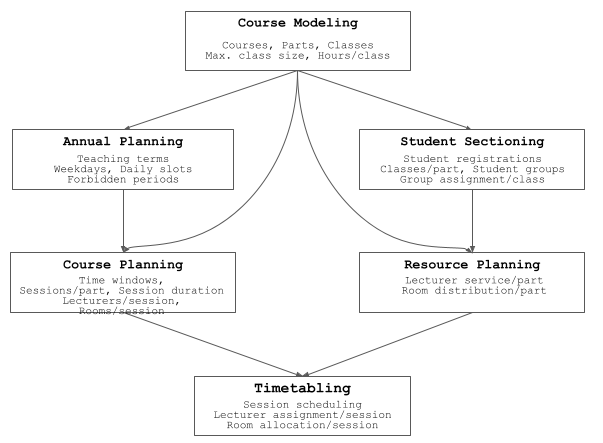
\includegraphics[scale= 0.4]{2022_JFPC_SLIDE/img/utp_workflow.png}
        \end{figure}
    %\end{minipage}
%    \hfill
%    \begin{minipage}{0.39\textwidth}
%    \begin{itemize}
%        %\item Multi-niveaux
%        \item Variant selon les pays et institutions
%        \item Modélisation complexe
%        \item Résolution difficile
%    \end{itemize}
%    \end{minipage}
    
    % \begin{minipage}{0.49\textwidth}
    %     \begin{itemize}
    %         %\item Caractéristiques
    %         %\begin{itemize}
    %             %
    %             %\item Différentes modalités de raisonnement (génération de solution, révision \ldots)
    %         %\end{itemize}
    %         \item Processus décisionnel
    %         \begin{itemize}
    %             \item Multi-niveaux (sectionnement, allocation, programmation \ldots)
    %             \item Différentes étapes, acteurs et échelles de temps
    %             \item Intrinsèquement dynamique (en continu avec des impondérables)
    %             \item Variant selon pays et institutions
    %         \end{itemize}
    %         \item Besoin d’outils flexibles d’aide à la décision
    %         \begin{itemize}
    %             \item Modélisation complexe (entités, règles \ldots)
    %             \item Résolution difficile (combinatoire, volumétrie)
    %         \end{itemize}
    %     \end{itemize}
    % \end{minipage}

\end{frame}

\begin{frame}{Construction d'EDT}
    \begin{minipage}{0.49\textwidth}
    \begin{itemize}
        %\item Multi-niveaux
        \item Sous-problèmes :
        \begin{itemize}
            \item Sectionnement d'effectifs
            \item Allocation de ressources
            \item Programmation de séances
        \end{itemize}
        \item Modélisation complexe
    \end{itemize}
\end{minipage}
    \begin{minipage}{0.49\textwidth}
    \begin{itemize}
        \item Volumétrie et combinatoire
        \item Sous-tend différents calculs :
        \begin{itemize}
            \item Génération d'EDT ex-nihilo
            \item Construction incrémentale
            \item Révision / réparation
        \end{itemize}
    \end{itemize}
\end{minipage}
\vspace{1cm}
    \begin{itemize}
   \item État de l'art 
   \vspace{-0.5cm}
\end{itemize}
   \begin{table}[!ht]
        \scriptsize
        \begin{tabular}{|c|c|c|c|}
             %\cline{1-4}
             \hline
             Problème & Domaine d'application & Schémas &  Méthode de résolution \\
            \hline
            \hline
             UCTP & Université & ITC-2019 \cite{2018_muller_PATAT} (XML) & SAT\cite{2021_lemos_TR}, ILP\cite{2014_aizam_NACO,2016_ober_PATAT},   \\
              \cline{1-3}
             STP & Collège/lycée & XHSST-2014 \cite{2012_ahmadi_AOR} (XML) & PPC\cite{1998_goltz_INAP,2006_gavalleni,2007_abdennadher_SBH}  \\
             \cline{1-3}
             ETP & Examen & ITC-2007 & Métaheuristiques        \cite{2010_hao_EJOR,2010_mushi_AJST,2019_jawa_JIM} \\
             \hline
        \end{tabular}
        
        \label{tab:my_label}
        
    \end{table}
    \vspace{-0.5cm}
    \begin{itemize}
       \item[] 
        %\begin{itemize}
        %\item Problèmes connexes BACP, NRP 
        %\item Problèmes connexes RCPSP, NRP 
        %\item[]
        \item Problèmes connexes : équilibrage de maquettes (BACP), sectionnement d'effectifs (SSP), allocation de tuteurs post-programmation (TAP)
        %\end{itemize}
    \end{itemize}

\end{frame}

\begin{frame}{Schéma de la compétition ITC-2019 \cite{2018_muller_PATAT}}

    \begin{itemize}
        \item Schéma le plus proche de nos besoins
        \item Caractéristiques du schéma 
        \begin{itemize}
            \item Décomposition hiérarchique des cours (parties, classes, séances)
            \item Regroupement des étudiants d'un cours dans une ou plusieurs classes 
            \item Classe à séances périodiques et de même durée
            \item Périodicité et durée de séances à déterminer par classe
            \item Catalogue de contraintes dédiées
            \item Optimisation multi-critères
        \end{itemize}
    \end{itemize}

    \begin{itemize}
        \item Ce qui n'est pas modélisable 
            \begin{itemize}
                \item Enseignants et services
                \item Séances multi-salles / multi-enseignants
                \item Salles multi-classes
                \item Salles virtuelles, salles obligatoires
                \item Programmation ``à la séance''
            \end{itemize}
    \end{itemize}
\end{frame}
\begin{frame}{Approche}
\begin{itemize}
    %\item Un langage pour une classe de problème d'EDT
    \item Formalisation et langage dédié pour une classe d'instances d'EDT : le problème \textbf{UTP}
    %\item Encodage du langage en XML : langage \textbf{XUTP}
    \item Modélisation et résolution PPC/CLP
    \item Implémentation du langage en XML et conversion vers JSON/DZN
\end{itemize}
    \begin{figure}
        \centering
        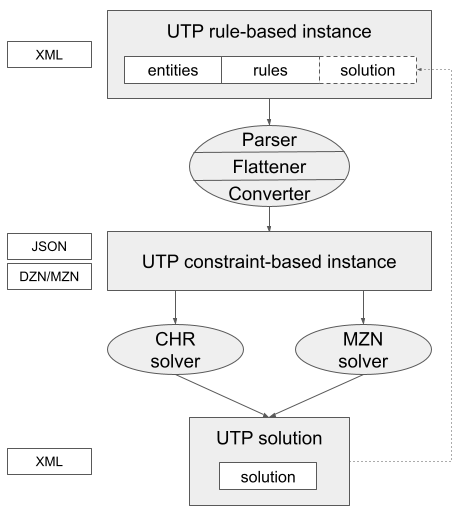
\includegraphics[width=5cm,height=5.2cm]{2022_JFPC_SLIDE/img/utp_toolchain.png}
    \end{figure}
\end{frame}

%==============

% \begin{frame}{Classes de problèmes d'emplois du temps}
% \begin{itemize}
%     \item Génération d'emplois du temps
%     \begin{itemize}
%         \item UCTP (University Course Timetabling Problem)
%         \item STP (School Timetabling Problem) 
%         \item ETP (Examination Timetabling Problem) 
%     \end{itemize}
%     \item Problèmes connexes :
%         \begin{itemize}
%             \item BACP (Balanced Academic Curriculum Problem)
%             \item TAP (Tutor Allocation Problem)
%             %\item RAP (Room Assignment Problem)
%             \item SSP (Student Sectionnement Problem)
%             \item RCPSP (Resource-Constrained Project Scheduling Problem)
%             \item NRP (Nurse Rostering Problem)
%         \end{itemize}
% \end{itemize}
% \end{frame}

%==============

% \begin{frame}{Modélisation}
% \begin{itemize}
%     \item Schémas de représentation : 
%         \begin{itemize}
%             \item Modèle ITC-2019 \cite{2018_muller_PATAT} format XML\footnote{\url{https://www.itc2019.org/}}
%             \item Modèle ITC-2007
%             \item Modèle XHSTT-2014 \cite{2012_ahmadi_AOR} format XML \footnote{\url{http://jeffreykingston.id.au/khe/}}
%         \end{itemize}
%     \item Variations entre modèles :
%     \begin{itemize}
%         \item Représentation des ressources
%         \item Représentation des cours
%         \item Représentation temporelle
%         \item Déclaration des contraintes 
%     \end{itemize}
% \end{itemize}
% \end{frame}

%==============

% \begin{frame}{Résolution}
% \begin{itemize}
%     \item Approches exactes :
%     \begin{itemize}
%         \item  ILP \cite{2014_aizam_NACO,2016_ober_PATAT}, MILP \cite{2012_alefragis_,2022_nurul_MJFAS}
%         \item  SAT \cite{2021_lemos_TR}, ASP \cite{2019_banbara_AOR}
%         \item  PPC \cite{1998_goltz_INAP,2006_gavalleni,2007_abdennadher_SBH}, CLP \cite{2007_abdennadher_SBH}
%     \end{itemize}
%     \item Méthodes approchées : 
%         \begin{itemize}
%             \item Algorithmes évolutionnaires \cite{2009_bratkovi_SBH}
%             \item Recherche tabou \cite{2010_hao_EJOR,2010_mushi_AJST}
%             \item Recuit simulé \cite{2006_bai_,2019_jawa_JIM}
%             \item Colonies de fourmis \cite{2019_mazlan_IJECS}
%             \item Hyper-heuristiques \cite{2015_ahmed_ESA}
%         \end{itemize}
% \end{itemize}
% \end{frame}

%==============
%===============================
%==============

%\begin{frame}{Chaîne de traitement}

%  \begin{minipage}{.53\textwidth}
%     \begin{itemize}
%         \item Parseur
%             \begin{itemize}
%                 \item Valide l'instance
%                 %\item Graphe des contraintes
%             \end{itemize}
%         \item Générateur
%             \begin{itemize}
%                 \item Construit les e-maps
%                 \item Génère les contraintes
%             \end{itemize}
%         \item Encodeur
%             \begin{itemize}
%                 \item Encode les contraintes générées
%                 \item Convertit au format attendu par les solveurs (JSON,DZN)
%             \end{itemize}
%     \end{itemize}
%  \end{minipage}
%   \begin{minipage}{0.45\textwidth}

%\setbeamercolor{block body}{bg=black!65}
    %\begin{figure}
      %  \centering
        %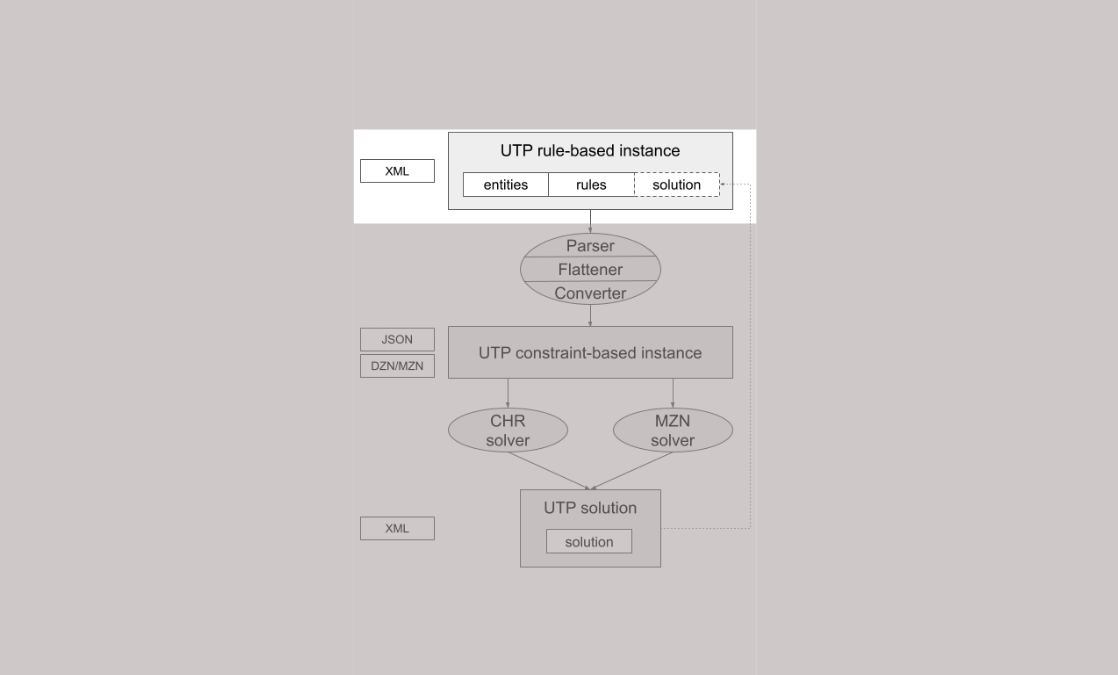
\includegraphics[scale = 0.4]{2022_JFPC_SLIDE/img/grisedFlowUTP.png}
     %   \label{fig:toolchain}
    %\end{figure}
        % \end{minipage}
%\end{frame}

\section{Un langage dédié pour une classe d'EDT}
%==============

%==============

\begin{frame}{Le problème UTP}
    
    \begin{minipage}[t]{0.49\textwidth}
    \begin{itemize}
        \item Dimensions
        \begin{itemize}
            \item Temps
            \item Effectif
            \item Nombre de séances
        \end{itemize}
        \item Entités
        \begin{itemize}
            \item Éléments de cours
            \item Ressources
        \end{itemize}

    \end{itemize}
    \end{minipage}
    \hfill
    \begin{minipage}[t]{0.49\textwidth}
    \begin{itemize}
        \item Règles
        \begin{itemize}
            \item Éligibilité, capacité et distribution des ressources
            \item Temporalité, allocation, sectionnement
            %\item Utilise un catalogue de contrainte EDT
        \end{itemize}
        \item Pré-affectation optionnelle
        \begin{itemize}
        \item Décisions de sectionnement, allocation, programmation
            %\item Partielle ou totale
            %\item Consistante ou inconsistante
        \end{itemize}
    \end{itemize}

    \end{minipage}
    \vspace{1cm}
        \begin{itemize}
        \item Langage de règles fondé sur un catalogue de prédicats EDT  \item Pas d'optimisation \lbrack dans cette version\rbrack
        \item Aucun pré-requis sur la pré-affectation
    \end{itemize}
\end{frame}

% \begin{frame}{Le langage dédié XUTP}
%   \begin{minipage}[t]{0.33\textwidth}
%       \begin{itemize}
%         \item[1] Encodage d'instance à base de règle
%     \end{itemize}
%   \end{minipage}
%   \begin{minipage}[t]{0.32\textwidth}
%       \begin{itemize}
%         \item[2] Conversion (flattening) des règles en contraintes
%     \end{itemize}
%   \end{minipage}
%   \begin{minipage}[t]{0.33\textwidth}
%       \begin{itemize}
%         \item[3] Encodage de l'instance à base de contraintes
%     \end{itemize}
%   \end{minipage}

%     \begin{figure}
%         \centering
%         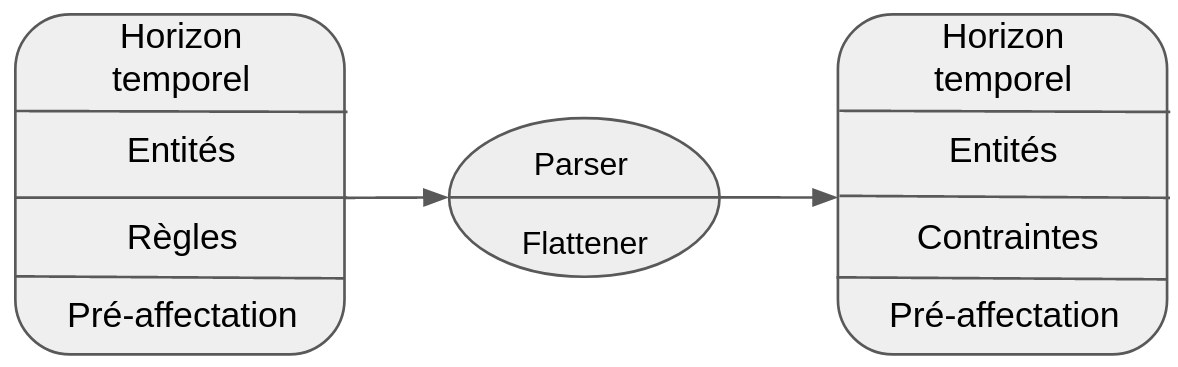
\includegraphics[scale=0.35]{2022_JFPC_SLIDE/img/flattenneritout.png}
%         \label{fig:xutp}
%     \end{figure}
% \end{frame}

%==============

\begin{frame}{Modèle d'entités}
% \begin{minipage}{0.33\textwidth}
%     \begin{itemize}
%         \item Maquette :
%         \begin{itemize}
%             \item Cours
%             \item Parties de cours
%             \item Classes
%             \item \lbrack Séances\rbrack
%         \end{itemize}
%     \end{itemize}
% \end{minipage}
% \begin{minipage}{0.3\textwidth}
%      \begin{itemize}
%         \item Ressources :
%             \begin{itemize}
%                 \item Salles
%                 \item Enseignants
%                 \item Étudiants
%                 \item \lbrack Groupes\rbrack
%             \end{itemize}
%     \end{itemize}
% \end{minipage}
% \begin{minipage}{0.33\textwidth}
%      \begin{itemize}
%         \item Horizon temporel :
%             \begin{itemize}
%                 \item Semaine
%                 \item Jour
%                 \item Créneaux à la minute
%             \end{itemize}
%     \end{itemize}
% \end{minipage}
    \begin{itemize}
        \item Horizon de temps à 3 niveaux
        \item Entités : éléments de maquette de formations, ressources
        \item Contraintes de domaine et de distribution de ressources
    \end{itemize}
    \begin{figure}
        \centering
        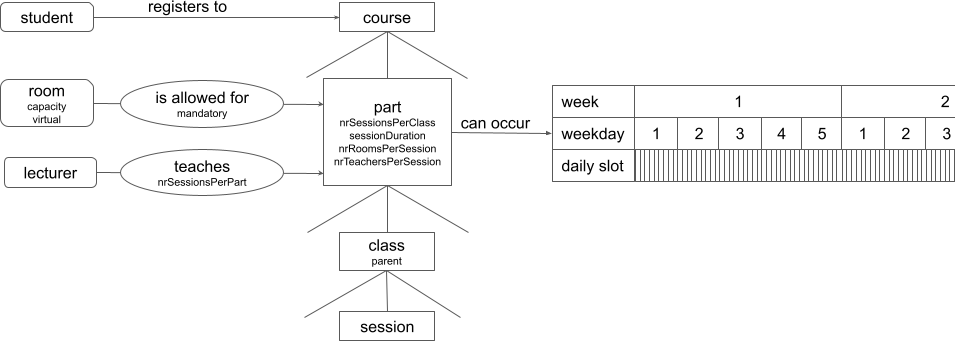
\includegraphics[scale = 0.33]{img/utp_entity_model.png}
        \label{fig:entities}
    \end{figure}
    \begin{itemize}
        \item Séances ordonnées par classe
    \end{itemize}
\end{frame}
%==============

\begin{frame}{Modèle d'entités : exemple}
        \begin{figure}
        \centering
        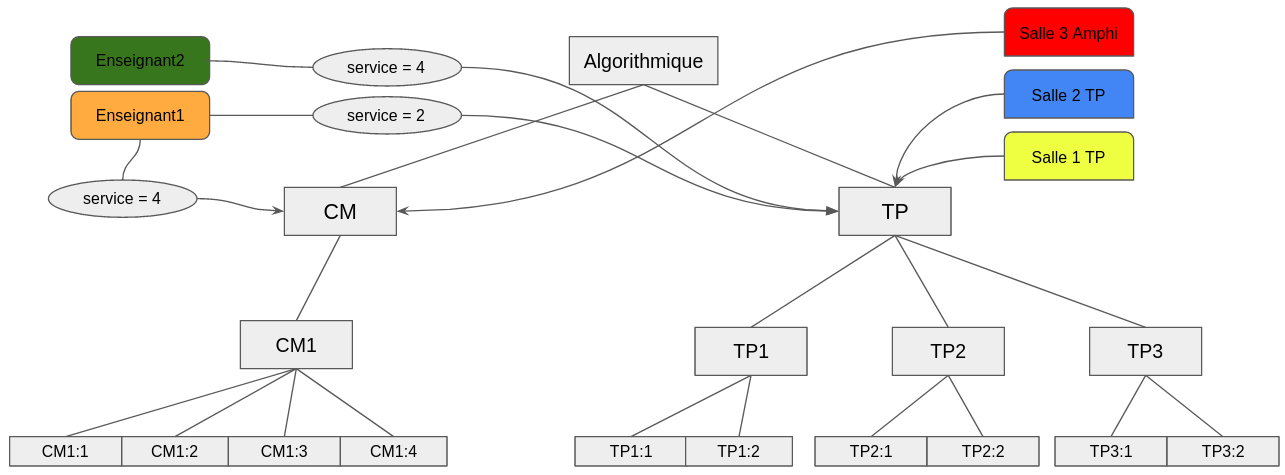
\includegraphics[scale=0.35]{2022_JFPC_SLIDE/img/treefrenchNature.png}
        \label{fig:my_tree_rule}
    \end{figure}
\end{frame}
%==============
 \begin{frame}[t]{Règles : exemple}
 \begin{itemize}
     \item ``Même semaine pour les premières séances de TP''
     \item ``Toujours la même salle pour la classe TP1''
     \item ``Séances de CM hebdomadaires sauf la deuxième séance''
     \item ``3 séances de CM précèdent la première séance de TP''
     \item ``enseignant2 absent le 01/01 de 10h à 20h''
     \item[]
 \end{itemize}
 Solution possible
  \begin{figure}
        \centering
        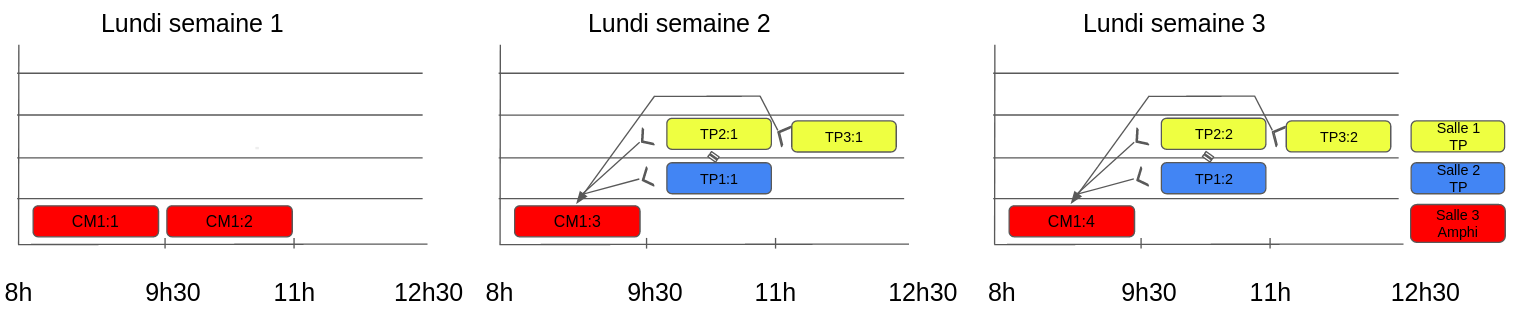
\includegraphics[width=11cm,height=3cm]{2022_JFPC_SLIDE/img/ordofrench3weeksJFPC2022example.png}
    \end{figure}
 \end{frame}
%==============

\begin{frame}{Catalogue de prédicats}
 \begin{itemize}
     \item Règles et contraintes s'appuient sur un catalogue de prédicats dédiés
     \item Prédicats d'arité fixe ou non, paramétrés ou non
    \end{itemize}

% \begin{minipage}{0.39\textwidth}
%
    \begin{table}[!ht]
        \centering
        \scriptsize
        \scalebox{1}{
        \begin{tabular}{|l|l|l|p{.4\textwidth}|}
            \hline
             Nom prédicat& Arité & Paramètres & Description \\
             \hline
            forbidden\_period         & 1         & oui   & Les séances ne peuvent pas débuter\\ 
            &&&dans la période donnée\\ \hline
            same\_rooms                & 1         & non    & Les séances ont lieu dans les mêmes salles\\ \hline
            sequenced                & $\geq2$   & non    & Les séances sont séquencées\\ \hline
            periodic                  & 1         & non    & Les séances démarrent les mêmes créneaux et jours de semaines successives \\ \hline
            ... &&& \\
            \hline
        \end{tabular}
        }
    \end{table}

%\end{minipage}
\end{frame}


\begin{frame}{Règles et contraintes}
%  \begin{overprint}
%    \onslide<1>

% \begin{itemize}
%     \item ``Toujours la même salle pour la classe TP1''
%     \item ``Séances de CM hebdomadaires sauf ma deuxième séance''
%     \item ``3 séances de CM précèdent les premières séances de TP''
%     \item ``enseignant2 absent le 01/01 de 10h à 20h''
% \end{itemize}
 
% \begin{minipage}{0.59\textwidth}
 \vspace{0.5cm}
 \begin{itemize}
     \item Une règle exprime en intension une conjonction de contraintes de même prédicat
%        \begin{itemize}
%        \item Prédicats d'arité quelconque et paramétrés ou non
%        \end{itemize}       
     \item Une contrainte porte sur une ou plusieurs paires associant chacune
        \begin{itemize}
        \item Un cours, une partie ou une classe à un ensemble de ses séances
            \begin{itemize}
            \item[=>] contraint toutes les séances
            \end{itemize}
        \item Ou une ressource à un ensemble de ses séances possibles
            \begin{itemize}
            \item[=>] contraint uniquement les séances qui lui seront allouées
            \end{itemize}
        \end{itemize}     
%     \item Une contrainte porte sur une ou plusieurs paires associant chacune une entité à un ensemble de séances
     
    \item[]  \hspace{1cm} $predicate(\langle \textcolor{red}{e_1},\textcolor{blue}{\{s_1,\ldots,s_n\}}\rangle, \ldots)$
    \item[] 
    \item Dans la portée d'une règle, chaque paire associe un type d'entités à un ensembles de séances filtrables, respectivement, par label/id et rang
%        \begin{itemize}
%        \item Filtrage selon type/label/id d'entités et rangs de séances
%        \end{itemize}  
    \item[]  \hspace{1cm} $predicate(\langle \textcolor{red}{(type,label|id)},\textcolor{blue}{\{rank_1,\ldots,rank_n\}}\rangle, \ldots)$
    \item[] 
    \item Génération des contraintes par instantiation de la portée de la règle
    \end{itemize}

% \vspace{-0.3cm}
%    \begin{figure}
%        \centering
%        \includegraphics[scale=0.25]{2022_JFPC_SLIDE/img/règleUTPPetitExemple.png}
%    \end{figure}
% \end{minipage} 
\end{frame}





\begin{frame}{Syntaxe des règles : exemple}

%    \onslide<2>
 \begin{itemize}
     \item ``Même semaine pour les premières séances de TP''
     \item ``Toujours la même salle pour la classe TP1''
     \item ``Séances de CM hebdomadaires sauf la deuxième séance''
     \item ``3 séances de CM précèdent la première séance de TP''
     \item ``enseignant2 absent le 01/01 de 10h à 20h''
 \end{itemize}
 \vspace{0.7cm}
    Règles UTP :
        \begin{itemize}
        \item same\_week(<\textcolor{red}{(partie,TP)},\textcolor{blue}{\{1\}}>))
        \item same\_rooms(<\textcolor{red}{(classe,TP1)},\textcolor{blue}{*}>))

        \item periodic(<\textcolor{red}{(classe,CM)},\textcolor{blue}{\{1,3-4\}}>,1,week)

        \item sequenced(<\textcolor{red}{(classe,CM)},\textcolor{blue}{\{3\}}>,<\textcolor{red}{(classe,TP)},\textcolor{blue}{\{1\}}>)

        \item forbidenPeriod(<\textcolor{red}{(enseignant,enseignant2)},\textcolor{blue}{*}>,600,1200)
    \end{itemize}
%    \end{overprint}
\end{frame}

%\begin{frame}{Conversion des règles}
%    % \begin{minipage}{0.49\textwidth}
%    \begin{itemize}
%        \item Conjonction de contraintes
%        \item Instancie les contraintes avec des couples entités, ensemble de séance
%        \item Ensemble de séance généré via des filtres, masques
%    \end{itemize}
%    % \end{minipage}
%    % \begin{minipage}{0.49\textwidth}
%
%    % \end{minipage}
%            \begin{figure}
%            \centering
%            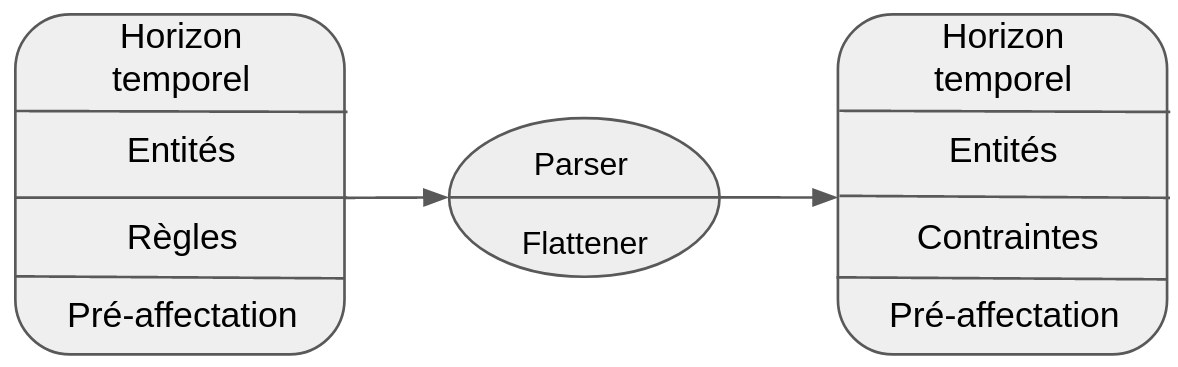
\includegraphics[scale=0.2]{2022_JFPC_SLIDE/img/flattenneritout.png}
%            \label{fig:my_label}
%        \end{figure}
%\end{frame}

%==============

% \begin{frame}{Modèle UTP : Règles}
%     \begin{itemize}
%         \item Une règle exprime en intension une conjonction de contraintes conditionnelles de même prédicat liant entités et séances possibles
%         \item Une contrainte porte sur une ou plusieurs paires (e-map) associant une entité et un ensemble de séances
%         \item la langage de règles intègre  un langage de sélecteurs permettant de cibler des types d'entités et des sous-ensembles de séances
%         \end{itemize} 
%     \begin{figure}
%         \centering
%         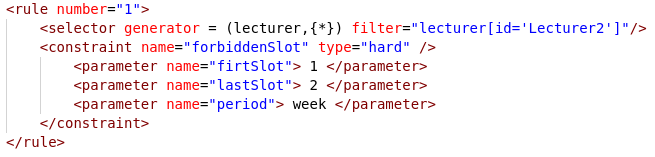
\includegraphics[scale= 0.55]{2022_JFPC_SLIDE/img/fragmentRule1.png}
%         \label{fig:rules1}
%     \end{figure}
% \end{frame}

\begin{frame}{Règles : exemple}
    \begin{figure}
        \centering
        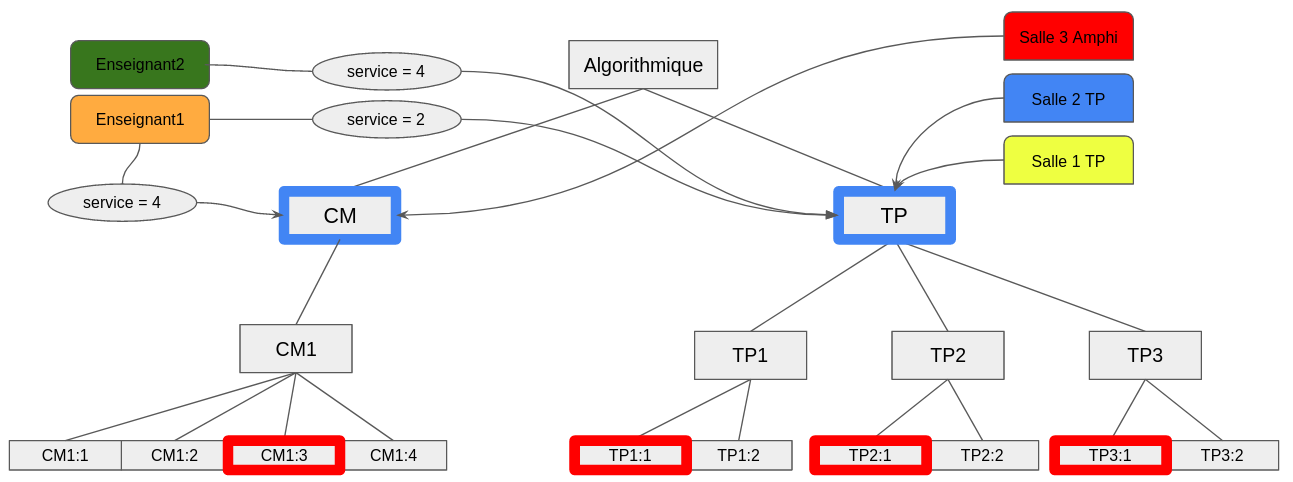
\includegraphics[scale= 0.3]{2022_JFPC_SLIDE/img/treesequencedJFPC2022.png}
        %\caption{Fonctionnement des règles}
        \label{fig:rules2}
    \end{figure}
    \begin{minipage}{0.5\textwidth}
    \begin{block}{\tiny Règle}
        \begin{itemize}
            \item {\tiny sequenced(<(classe,CM),\{3\}>,<(classe,TP),\{1\}>)} 
        \end{itemize}
    \end{block}
    \end{minipage}
    \hfill
    \begin{minipage}{0.45\textwidth}
     \begin{alertblock}{\tiny Contraintes}
        \begin{itemize}
        \item {\tiny sequenced(<CM1,\{3\}>,<TP1,\{5\}>)}
        \item {\tiny sequenced(<CM1,\{3\}>,<TP2,\{7\}>)}
        \item {\tiny sequenced(<CM1,\{3\}>,<TP3,\{9\}>)}
    
        \end{itemize}
        \end{alertblock}
    \end{minipage}
\end{frame}

\begin{frame}{Règles : exemple}
    \begin{figure}
        \centering
        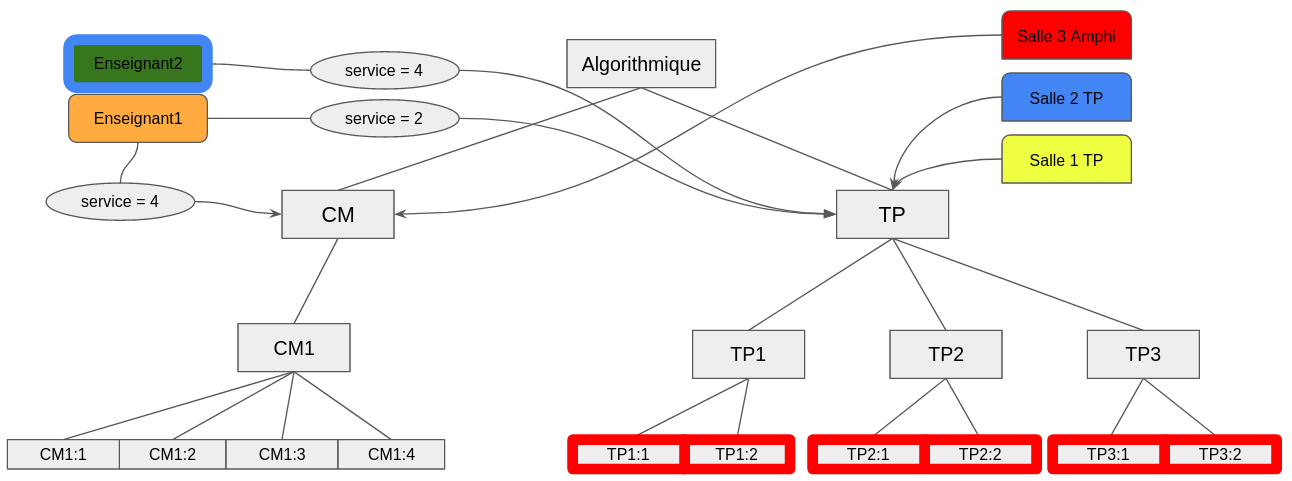
\includegraphics[scale= 0.3]{2022_JFPC_SLIDE/img/treefrenchforbidden.png}
        %\caption{Fonctionnement des règles}
        \label{fig:rules2}
    \end{figure}
    \begin{minipage}{0.45\textwidth}
    
    \begin{block}{\tiny Règle}
             {\tiny forbidden\_slot(<(enseignant,enseignant2),*>,600,1200)}
\end{block}
    \end{minipage}
    \hfill
    \begin{minipage}{0.45\textwidth}
    \begin{alertblock}{\tiny Contraintes}
        {\tiny forbidden\_slot(<enseignant2,\{5-10\}>,600,1200)   }

    \end{alertblock}
    \end{minipage}
\end{frame}

%==============


\begin{frame}{Modèle UTP : Pré-affectation}
    \begin{itemize}
        \item Modélise des décisions portant sur
        \begin{itemize}
            \item Sectionnement d'effectifs
            \item Allocations de ressources
            \item Ordonnancement de séances
        \end{itemize}
        
        \item[]
        \item Peut être 
        \begin{itemize}
            \item Vide, partielle ou totale
            \item Consistante ou inconsistante
        \end{itemize}
    \end{itemize}
\end{frame}
%==============
\section{Modélisation et résolution en CP/CLP}
%=============

%==============

% \begin{frame}{Résolution UTP : Ordonnancement}
%     \begin{itemize}
%     \item Variables entières
%     \item Contraintes d'ordonnancement
%         \begin{itemize}
%             \item Séquencement
%             \item Parallélisation
%             \item Répartition
%             \item Périodicité
%             \item Domaine
%         \end{itemize}
%     \end{itemize}
%         \begin{figure}
%             \centering
%             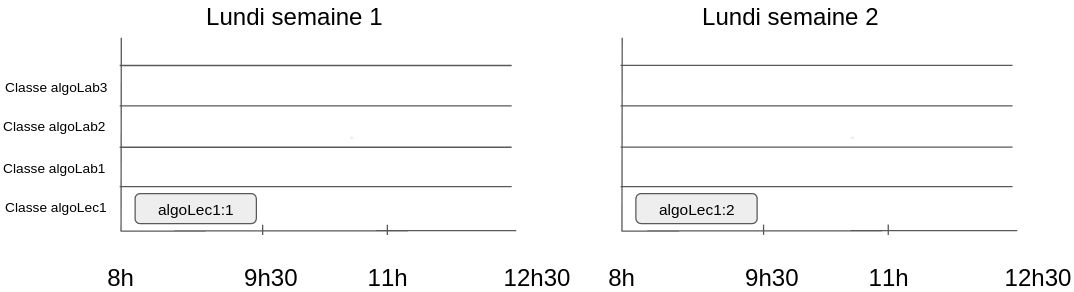
\includegraphics[scale = 0.29]{2022_JFPC_SLIDE/img/ordoJFPC2022_1.png}
%             \end{figure}
            
%             \begin{figure}
%             \hspace{5.7mm}
%             \centering
%             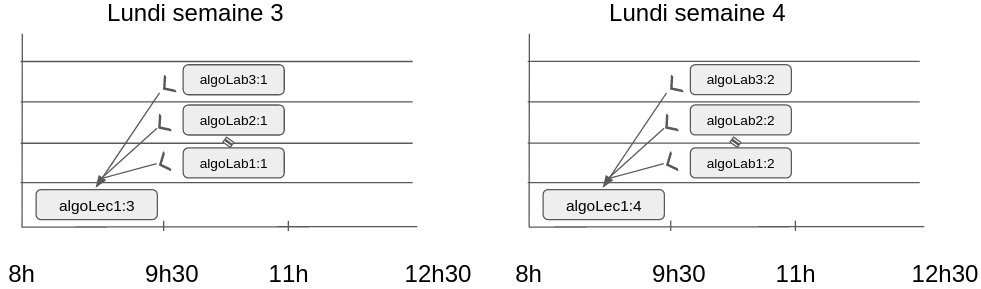
\includegraphics[scale = 0.29]{2022_JFPC_SLIDE/img/ordoJFPC2022_2.png}
%             \label{fig:ordo}
%         \end{figure}

% \end{frame}

\begin{frame}{Résolution UTP : ordonnancement cumulatif et disjonctif}
    \begin{minipage}{0.49\textwidth}
    \begin{itemize}
    \item Variables entières
    \item Contraintes temporelles
        \begin{itemize}
            \item Séquencement
            \item Parallélisation
            \item Répartition
            \item Périodicité
            \item Plages autorisées
        \end{itemize}
    \end{itemize}
    \end{minipage}
    \begin{minipage}{0.49\textwidth}
        \begin{itemize}
    \item Variables ensemblistes
    \item Contraintes d'allocation
        \begin{itemize}
            \item Cardinalité %\lbrack coeur \rbrack 
            \item Compatibilité/éligibilité %\lbrack coeur \rbrack
            \item Capacité
            \item Ressources cumulatives %\lbrack coeur \rbrack
            \item Ressources disjonctives %\lbrack règle \rbrack
        \end{itemize}
    \end{itemize}
    \end{minipage}
                \begin{figure}
            \centering
            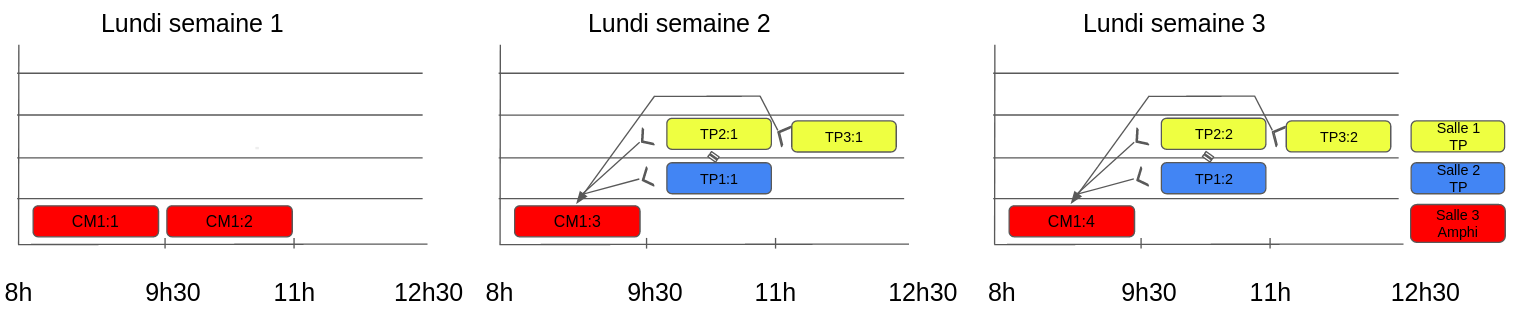
\includegraphics[width=11cm,height=3cm]{2022_JFPC_SLIDE/img/ordofrench3weeksJFPC2022example.png}
            \end{figure}
            \begin{itemize}
                \item Contraintes de sectionnement
            \end{itemize}
\end{frame}
%==============

% \begin{frame}{Résolution UTP : Ordonnancement cumulatif et disjonctif}
%     \begin{itemize}
%     \item Variables ensemblistes
%     \item Contraintes sur les ressources
%         \begin{itemize}
%             \item Contraintes de cardinalité %\lbrack coeur \rbrack 
%             \item Contraintes de domaine %\lbrack coeur \rbrack
%             \item Contraintes cumulatives %\lbrack coeur \rbrack 
%             \item Contraintes disjonctive %\lbrack règle \rbrack 

%         \end{itemize}
%     \end{itemize}
    
%             \begin{figure}
%             \centering
%             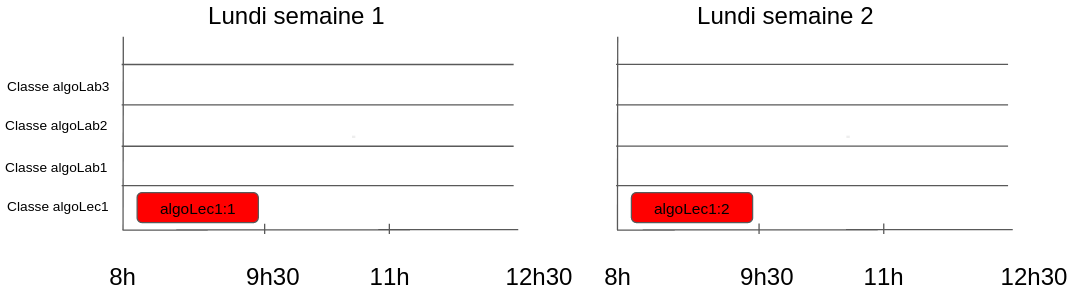
\includegraphics[scale = 0.29]{2022_JFPC_SLIDE/img/ordoJFPC2022Disjunct_1.png}
%             \end{figure}
            
%             \begin{figure}
%             \hspace{1cm}
%             \centering
%             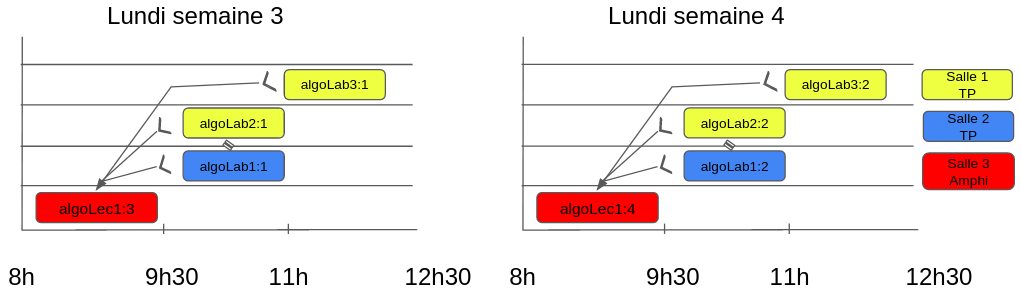
\includegraphics[scale = 0.29]{2022_JFPC_SLIDE/img/ordoJFPC2022Disjunct_2.png}
%             \label{fig:ordo}
%         \end{figure}

% \end{frame}

%==========

\begin{frame}{Programmes en CP et CLP}

 \begin{minipage}{0.2\textwidth}
 \end{minipage}
 \hfill
  \begin{minipage}{0.79\textwidth}
%  \centering
        \begin{itemize}
%        \item Traité comme un problème de satisfiabilité 
        \item Hypothèse : sectionnement pré-résolu
        \item[]
    \end{itemize}
 \end{minipage} 
 \vspace{1.5mm}
    \begin{columns}[c]
    %\begin{columns}
\begin{column}{0.5\textwidth}
Modèle Minizinc
\begin{itemize}
    \item Réification des variables d'allocation pour contraintes conditionnelles
    \item Contraintes globales
    \item Stratégie : allocation de ressources aléatoire puis ordonnancement par dichotomie (domain splitting)
\end{itemize}
\end{column}
%\hspace{-50pt}
\vrule{}
\begin{column}{0.50\textwidth}
Programme CHR++
\begin{itemize}
        \item Variable décisionnelle supplémentaire 
        \item Contraintes statiques, dynamiques
        \item Prédicats statiques, dynamiques
        \item Filtrage de domaine
        \item Utilisation du graphe disjonctif
\end{itemize}
\end{column}
\end{columns}

\end{frame}

%==============
%===============================
%==============
%==============
\section{Expérimentations et perspectives}
\begin{frame}{Premières expérimentations}
    \begin{itemize}
        \item Instance :
        \begin{itemize}
            \item Semestre 2 Licence 3 informatique université d'Angers
            \begin{itemize}
                \item 12 semaines, 5 jours, 1440 créneaux quotidien
                \item 9 cours, 25 parties de cours, 48 classes, 262 séances
                \item  67 étudiants, 8 salles, 12 enseignants
                \item 55 règles, 668 contraintes
            \end{itemize} 
            
            \item Solution obtenue en moins de 5s
        \end{itemize}
        \item[]
         \item Expérimentations en cours :
        \begin{itemize}
            \item Encodage de la L1 MI-MPC de l'université d'Angers
        \end{itemize}
    \end{itemize}
\end{frame}
%=============

% \begin{frame}{Perspectives}
%     \begin{minipage}{0.49\textwidth}
%         \begin{itemize}
%         \item Langage XUTP 
%             \begin{itemize}
%                 \item Rajouter une syntaxe générative
%                 \item Étendre le catalogue de prédicat
%                 \item Intégrer les événements
%               % \item Ajouter les événements
%             \end{itemize}
%         \item Modèles PPC
%             \begin{itemize}
%                 \item Implémenter les nouveaux prédicats
%                 \item Stratégies de recherche
%             \end{itemize}
%         \item Expérimentation 
%         \begin{itemize}
%             \item Passage à l'échelle
%             \item Réduction entre modèles (ITC vers UTP)
%         \end{itemize}
%         \item Reformulation 
%     \end{itemize}
%     \end{minipage}
%     \hfill
%     \begin{minipage}{0.49\textwidth}
%         \begin{itemize}
%         \item Réparation des emplois du temps
%             \begin{itemize}
%                 \item Approche par contraintes souples
%                 \item Algorithme de réparation (voisinage, symétrie,...) par optimisation et opérateurs dédiés
%             \end{itemize}
%         %\item Réécriture des instances 
%             %\begin{itemize}
%             %    \item Simplification de l'horizon temporelle
%             %    \item Simplification des variables ensemblistes
%             %    \item réécriture de contraintes cumulatives
%           % \end{itemize}
%         \item Traitement des sous problèmes
%         \begin{itemize}
%             \item Sectionnement des étudiants
%             \item Pré-affectation des enseignants
%         \end{itemize}
        
%     \end{itemize}
%     \end{minipage}
% \end{frame}

%==============

\begin{frame}{Conclusion}
    \begin{itemize}
    \item Langage dédié et modèles CP/CLP pour une classe de problèmes d'EDT
        % \item Objectif de résoudre les problèmes d'emplois du temps universitaire
            % \begin{itemize}
            %     \item Définition du langage XUTP et implémentation d'outils pour l'utiliser
            %     \item Résolution via des méthodes exactes
            %     \begin{itemize}
            %         \item Modèle CHR, MiniZinc
            %     \end{itemize}
            %     %\item Étudier des méthodes de réparation et de révision de solution.
            % \end{itemize}
        \item Perspectives 
        \begin{itemize}
            \item Étendre le catalogue des prédicats
            \item Gérer les préférences (optimisation)
            \item Expérimentations et passage à l'échelle
            \item Révision et réparation d'emplois du temps
        \end{itemize}
    \end{itemize}
    \begin{itemize}
        \item Spécifications, benchmarks \lbrack en construction\rbrack, sources : \url{https://ua-usp.github.io/timetabling/} 
    \end{itemize}
\end{frame}

%==============
%\printbibliography

%======================================================================
%======================================================================


\end{document}
